\documentclass[aspectratio=169, 12pt]{beamer}

% ======================
% PAQUETES
% ======================
\usepackage[spanish]{babel}
\usepackage[utf8]{inputenc}
\usepackage[T1]{fontenc}
\usepackage{amsmath}
\usepackage{amssymb}
\usepackage{graphicx}
\usepackage{hyperref}
\usepackage{xcolor}
\usepackage{listings}
\usepackage{booktabs}

% ======================
% TEMA Y COLORES
% ======================
\usetheme{Madrid}
\usecolortheme{default}
\setbeamertemplate{navigation symbols}{}
\setbeamertemplate{footline}[frame number]
\setbeamertemplate{frametitle}[default][center]

% Colores personalizados
\definecolor{eafit}{RGB}{0, 51, 102}
\definecolor{lightgray}{RGB}{240, 240, 240}
\setbeamercolor{frametitle}{bg=eafit, fg=white}
\setbeamercolor{section in head/foot}{bg=eafit, fg=white}

% ======================
% INFO GENERAL
% ======================
\title{Propensión al Consumo de Marihuana en Colombia}
\subtitle{Benchmark Econométrico, Modelos de \textit{Machine Learning} e Interpretabilidad SHAP}

\author[Tupaz, Quintero, Rodrigues]{
Santiago Tupaz, Moisés Quintero, Vanessa Rodrigues
}

\institute[EAFIT]{
Universidad EAFIT, Programa de Economía \\[0.3cm]
{\small Profesora Supervisora: Paula María Almonacid Hurtado}
}

\date{12 de mayo de 2026}

% ======================
% DOCUMENTO
% ======================
\begin{document}

% Portada
{\setbeamertemplate{footline}{}
\frame{\titlepage}}



% Introducción y Motivación
\section{Introducción}

\begin{frame}
\frametitle{Contexto y motivación}
\begin{itemize}
    \item \textbf{Tendencia global}: más de 40 países han legalizado el cannabis en alguna forma.
    \item \textbf{Colombia}: el debate sobre regulación incorpora hoy preguntas económicas concretas (tamaño de mercado, base tributaria, política preventiva).
    \item \textbf{Pregunta previa}: antes de cualquier simulación fiscal, hay que caracterizar empíricamente \textbf{quién consume} y \textbf{con qué propensión}.
    \item \textbf{Insumo natural}: la Encuesta Nacional de Consumo de Sustancias Psicoactivas (ENCSPA).
\end{itemize}
\end{frame}

\begin{frame}
\frametitle{Brecha que aborda este trabajo}
\begin{itemize}
    \item Pocos modelos comparan rigurosamente \textbf{benchmark econométrico vs.\ \textit{machine learning}} en este dominio para Colombia.
    \item Escasa discusión estructurada de \textbf{ética y sesgos} en estudios de consumo de drogas con datos de encuesta.
    \item Necesidad de \textbf{interpretabilidad} (no sólo precisión) cuando el modelo se usa para política pública.
\end{itemize}
\vspace{0.3cm}
\textbf{Nuestra contribución}: pipeline reproducible + comparación honesta + interpretabilidad SHAP + frontera ética explícita.
\end{frame}

\begin{frame}
\frametitle{¿Por qué importa?}
\begin{columns}
\column{0.5\textwidth}
\textbf{Dimensión económica:}
\begin{itemize}
    \item Tamaño potencial del mercado
    \item Base tributaria si se legaliza
    \item Elasticidad-precio del segmento
\end{itemize}

\column{0.5\textwidth}
\textbf{Dimensión social:}
\begin{itemize}
    \item Focalización de prevención
    \item Reducción del estigma vía datos
    \item Uso responsable de IA en política
\end{itemize}
\end{columns}
\end{frame}

% Pregunta de Investigación
\section{Pregunta de Investigación}

\begin{frame}
\frametitle{Pregunta central}
\begin{center}
\large
\textbf{¿Qué factores sociodemográficos observables se asocian con la probabilidad de reportar consumo de marihuana en los últimos doce meses en Colombia, y cuánto mejora la predicción al pasar de un benchmark econométrico a modelos de \textit{machine learning}?}
\end{center}
\vspace{0.4cm}
\normalsize
Componentes:
\begin{enumerate}
    \item \textbf{Descriptivo-causal}: signo, magnitud y estabilidad de los predictores.
    \item \textbf{Predictivo}: ganancia del ML sobre el lineal manteniendo el mismo \textit{feature set}.
\end{enumerate}
\end{frame}

\begin{frame}
\frametitle{Variable objetivo y unidad de análisis}
\textbf{Variable dependiente:} \(\texttt{propension\_12m}\in\{0,1\}\) — reportó consumo de marihuana en los últimos 12 meses (base limpia, derivada de K\_03 + señales auxiliares).

\vspace{0.3cm}
\textbf{Unidad de análisis:} individuo encuestado (ENCSPA).

\vspace{0.3cm}
\textbf{Tipo de problema:} clasificación binaria.

\vspace{0.4cm}
\textit{Nota crítica}: la construcción de \texttt{propension\_12m} difiere de \texttt{K\_03} \textit{raw} en 898 casos. Se documenta como limitación y se atiende con un análisis de robustez (Y estricta = K\_03=1).
\end{frame}

\begin{frame}
\frametitle{Objetivos}
\textbf{General:} construir un pipeline reproducible que compare benchmark econométrico y \textit{machine learning} para la propensión al consumo, con interpretabilidad y reflexión ética explícitas.

\vspace{0.4cm}
\textbf{Específicos:}
\begin{enumerate}
    \item Integrar y limpiar la base de la ENCSPA con módulos sociodemográficos.
    \item Estimar benchmark MCO/Probit y modelos ML comparables.
    \item Validar con CV-10 y tunear hiperparámetros del modelo final.
    \item Interpretar con valores SHAP y verificar robustez.
    \item Discutir sesgos, ética y usos legítimos del modelo.
\end{enumerate}
\end{frame}

% Metodología
\section{Metodología}

\begin{frame}
\frametitle{Datos y fuentes — 5 módulos integrados}
\begin{columns}[T]
\column{0.52\textwidth}
\textbf{Fuentes}
\begin{itemize}
\item Base limpia de consumo (cap. K)
\item Módulo \texttt{personas} (sexo, edad)
\item Módulo \texttt{d2} (educación, hijos)
\item Módulo \texttt{g} (red social, actitud)
\item Módulo \texttt{d} (laboral, salud, percepción)
\end{itemize}

\column{0.44\textwidth}
\textbf{Cobertura}
\begin{itemize}
\item \(n=3\,982\) individuos
\item 16 features, 0\% nulos (salvo \texttt{regimen\_salud}: 11.2\%)
\item \texttt{consumo\_12m}: 1\,719 positivos
\item Precio: submuestra exploratoria ($n{\approx}755$)
\end{itemize}
\end{columns}
\vspace{0.3cm}
\textit{Decisión}: ML sobre la muestra amplia sin precio.
\end{frame}

\begin{frame}
\frametitle{Pipeline reproducible}
\begin{enumerate}
\item \texttt{python -m cannabis\_tax.cli pipeline}: limpieza, validación y construcción de la base modeladora.
\item Notebook 01: EDA + benchmark MCO/Probit.
\item Notebook 03: entrenamiento RF, XGBoost, GBM.
\item Notebook 05: CV-10, búsqueda de hiperparámetros, selección del modelo final.
\item Notebook 06: SHAP + robustez + ética.
\end{enumerate}
\vspace{0.3cm}
\textit{Tests}: \texttt{make test} corre la suite unitaria.
\end{frame}

\begin{frame}
\frametitle{Benchmark econométrico}
\textbf{MCO (LPM)}:
\[
y_i = \beta_0 + \beta_2 edad_i + \beta_3 edad_i^2 + \beta_4 mujer_i + \beta_5 educacion_i + u_i
\]
con errores HC1.

\vspace{0.3cm}
\textbf{Probit}:
\[
\Pr(y_i=1\mid X_i) = \Phi(\alpha_0 + \alpha_2 edad_i + \alpha_3 edad_i^2 + \alpha_4 mujer_i + \alpha_5 educacion_i)
\]
con efectos marginales promedio.

\vspace{0.3cm}
\textit{Roles}: referencia interpretable y punto de comparación.
\end{frame}

\begin{frame}
\frametitle{Feature set ampliado — 16 variables}
\centering
\footnotesize
\begin{tabular}{ll}
\toprule
\textbf{Grupo} & \textbf{Variables} \\
\midrule
Demográficas base & edad, edad², sexo, educación \\
Estructura familiar & n\_hijos \\
Red social (G\_01, G\_02) & familiares\_consumen, amigos\_consumen \\
Actitud (G\_04, G\_09) & probaria\_sustancias, cannabis\_medicinal \\
Situación socioeconómica (D\_02, D\_07) & actividad\_laboral, regimen\_salud \\
Salud mental PHQ-2 (D\_09, D\_10) & sintomas\_depresivos, anhedonia \\
Percepción de riesgo (D\_11\_F, D\_11\_G) & riesgo\_marihuana\_ocasional/frecuente \\
\bottomrule
\end{tabular}
\vspace{0.3cm}
\\
\small Todos con 0\% de nulos salvo \texttt{regimen\_salud} (11.2\%). Categóricas con \textit{one-hot encoding}.
\end{frame}

\begin{frame}
\frametitle{Modelos de Machine Learning}
\begin{itemize}
    \item \textbf{Random Forest}: \textit{bagging}, 300 árboles, \texttt{max\_depth=7}.
    \item \textbf{XGBoost}: \textit{boosting} secuencial, ponderado por prevalencia.
    \item \textbf{Gradient Boosting (sklearn)}: \textit{boosting} conservador, \texttt{max\_depth=3}.
\end{itemize}
\vspace{0.3cm}
\textbf{Reglas de comparación}:
\begin{itemize}
    \item \textit{Feature set} ampliado de 16 variables (ver tabla anterior).
    \item Mismo \texttt{train/test split} estratificado (\texttt{random\_state=42}).
    \item Métricas: Accuracy, AUC-ROC, F1, CV AUC (5 y 10 folds).
\end{itemize}
\end{frame}

\begin{frame}
\frametitle{Validación y selección}
\begin{enumerate}
    \item \textbf{CV-10}: estabilidad y solapamiento entre modelos.
    \item \textbf{Curvas de aprendizaje}: control de \textit{overfitting}.
    \item \textbf{\texttt{RandomizedSearchCV}}: 60 combinaciones × 5 folds sobre el GBM.
    \item \textbf{Criterios}: AUC-ROC, F1, brecha train-validation, plausibilidad económica.
\end{enumerate}
\vspace{0.3cm}
\textit{No se evalúa sólo precisión}: la argumentación pesa tanto como el número.
\end{frame}

% Resultados
\section{Resultados}

% ── Slide 1: Benchmark ──
\begin{frame}
\frametitle{Benchmark econométrico — una referencia exigente}
\small
Con sólo 4 variables demográficas, los modelos lineales fijan una barra alta:

\vspace{0.3cm}
\centering
\scriptsize
\begin{tabular}{lrrrr}
\toprule
Modelo & Accuracy & AUC-ROC & F1 & CV AUC (5-fold) \\
\midrule
MCO (LPM) & 0.6611 & 0.7033 & 0.5823 & — \\
Probit     & 0.6611 & 0.7027 & 0.5817 & 0.6648 \\
\midrule
Random Forest     & 0.6397 & 0.6600 & 0.5689 & 0.6316 \\
Gradient Boosting & 0.6373 & 0.6947 & 0.5511 & 0.6667 \\
\textbf{GBM Tuneado} & \textbf{0.6573} & \textbf{0.6959} & \textbf{0.5891} & \textbf{0.6714} \\
\bottomrule
\end{tabular}

\vspace{0.3cm}
\flushleft
\scriptsize
\textbf{Hallazgo}: con hiperparámetros por defecto, el ML \textit{no} supera al benchmark.\\
El GBM tuneado apenas gana en CV5: $+0.007$ sobre Probit, $+0.005$ sobre AUC de prueba.\\
El benchmark no es formalidad; es una \textbf{restricción activa}.
\end{frame}

% ── Slide 2: Por qué el ML no gana por defecto ──
\begin{frame}
\frametitle{¿Por qué el ML no supera al benchmark por defecto?}
\begin{columns}[T]
\column{0.55\textwidth}
\centering
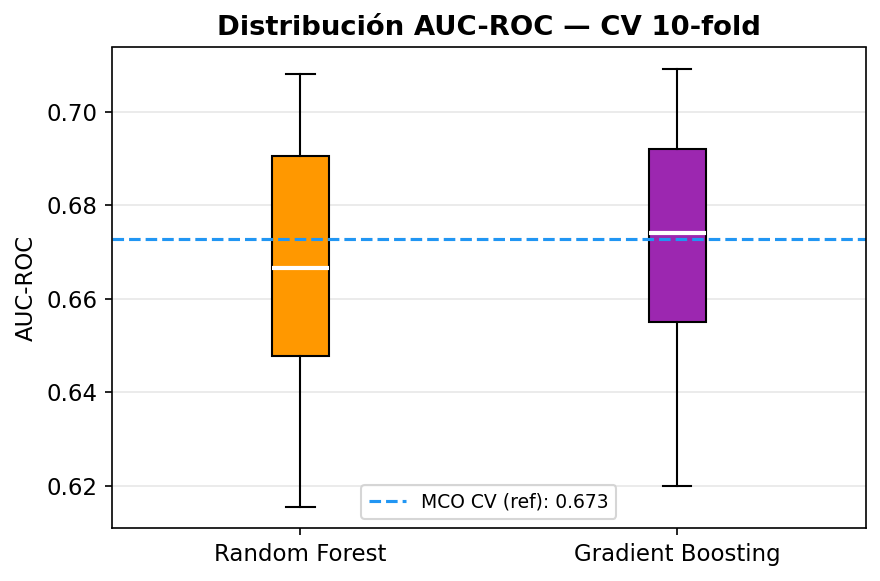
\includegraphics[width=\textwidth]{../figures/cv_10fold_boxplot.png}
\scriptsize CV-10 — solapamiento sustancial entre modelos

\column{0.42\textwidth}
\small
\textbf{Interpretación}:
\begin{itemize}
    \item Relación aproximadamente aditiva en 4 variables $\Rightarrow$ MCO minimiza sesgo.
    \item ML sin regularización paga varianza sin ganancia de sesgo.
    \item Las cajas de CV-10 se solapan: diferencias no robustas.
    \item El CV5 AUC del GBM tuneado (0.671) apenas supera al Probit (0.665).
\end{itemize}
\vspace{0.2cm}
\textit{La ganancia real vendrá de ampliar el feature set.}
\end{columns}
\end{frame}

% ── Slide 3: Tuning GBM (4-var) ──
\begin{frame}
\frametitle{Búsqueda de hiperparámetros sobre 4 variables — 300 evaluaciones}
\small
\textbf{Estrategia}: \texttt{RandomizedSearchCV}, 60 combinaciones × 5 folds estratificados.

\vspace{0.2cm}
\begin{columns}[T]
\column{0.42\textwidth}
\centering
\footnotesize
\begin{tabular}{lr}
\toprule
Hiperparámetro & Valor óptimo \\
\midrule
\texttt{n\_estimators} & 157 \\
\texttt{max\_depth} & 2 \\
\texttt{learning\_rate} & 0.042 \\
\texttt{subsample} & 0.972 \\
\texttt{min\_samples\_leaf} & 26 \\
\texttt{max\_features} & \texttt{log2} \\
\bottomrule
\end{tabular}

\column{0.55\textwidth}
\small
\textbf{Patrón interpretable}:\\[0.2cm]
Árboles muy superficiales (\texttt{depth=2}) + tasa baja + submuestra alta = \textbf{regularización agresiva}.

El ML gana no por mayor complejidad, sino por mejor control del compromiso \textbf{sesgo-varianza}.

\vspace{0.2cm}
\textit{Pero la ganancia sobre el benchmark es marginal con sólo 4 variables.}
\end{columns}
\end{frame}

% ── Slide 4: Modelo ampliado — resultados ──
\begin{frame}
\frametitle{Modelo ampliado — 16 variables, 7 grupos teóricos}
\small
\textbf{Muestra efectiva}: $n = 3\,401$ (eliminación por lista; 11.2\% de nulos en \texttt{regimen\_salud}).

\vspace{0.25cm}
\centering
\scriptsize
\begin{tabular}{lrrrr}
\toprule
Modelo (16 feat.) & $n$ & Accuracy & AUC-ROC & CV5 AUC \\
\midrule
Random Forest          & 3\,401 & 0.6397 & 0.6519 & $0.677 \pm 0.018$ \\
Gradient Boosting      & 3\,401 & 0.6490 & 0.6949 & $0.699 \pm 0.019$ \\
GBM Tuneado (16 vars)  & 3\,401 & 0.6505 & 0.6990 & $0.704 \pm 0.021$ \\
\textbf{RF Tuneado (16 vars)}   & \textbf{3\,401} & \textbf{0.6667} & \textbf{0.6995} & $\mathbf{0.703 \pm 0.007}$ \\
\midrule
\textit{Ref.: Probit (4 feat.)} & \textit{3\,980} & — & \textit{0.7027} & \textit{0.665} \\
\bottomrule
\end{tabular}

\vspace{0.3cm}
\flushleft
\scriptsize
\textbf{Lectura clave}: el CV5 AUC del RF Tuneado (0.703) supera al benchmark Probit (0.665) en \textbf{+0.038} y al GBM tuneado (4 vars) en \textbf{+0.032}. La varianza del RF ($\pm 0.007$) es \textbf{tres veces menor} que la del GBM tuneado ($\pm 0.021$), confirmando su estabilidad de generalización.
\end{frame}

% ── Slide 5: ¿Por qué RF? Justificación ──
\begin{frame}
\frametitle{Selección del modelo — ¿por qué RF Tuneado?}
\small
\textbf{Criterio}: menor varianza de CV5 + brecha \textit{train-test} controlada + máximo CV5 AUC.

\vspace{0.25cm}
\begin{columns}[T]
\column{0.48\textwidth}
\centering
\textbf{Hiperparámetros (RF regularizado):}\\[0.2cm]
\footnotesize
\begin{tabular}{lr}
\toprule
Parámetro & Valor \\
\midrule
\texttt{n\_estimators} & 400 \\
\texttt{max\_depth} & 15 \\
\texttt{max\_features} & 0.30 \\
\texttt{min\_samples\_leaf} & 25 \\
\texttt{min\_samples\_split} & 10 \\
\texttt{bootstrap} & True \\
\bottomrule
\end{tabular}

\column{0.50\textwidth}
\small
\textbf{Diagnóstico de ajuste}:\\[0.1cm]
\begin{itemize}
    \item AUC train = 0.760, AUC test = 0.700
    \item Brecha = \textbf{0.060} (antes 0.094)
    \item Curva de aprendizaje \textbf{estable}: no memorización
    \item CV5 $\pm 0.007$: la menor de todos los modelos
\end{itemize}
\vspace{0.1cm}
\textit{Regularización explícita: profundidad + hojas mínimas + bagging.}
\end{columns}
\end{frame}

% ── Slide 6: Curva de aprendizaje RF ──
\begin{frame}
\frametitle{Curva de aprendizaje — RF Tuneado (16 variables)}
\centering
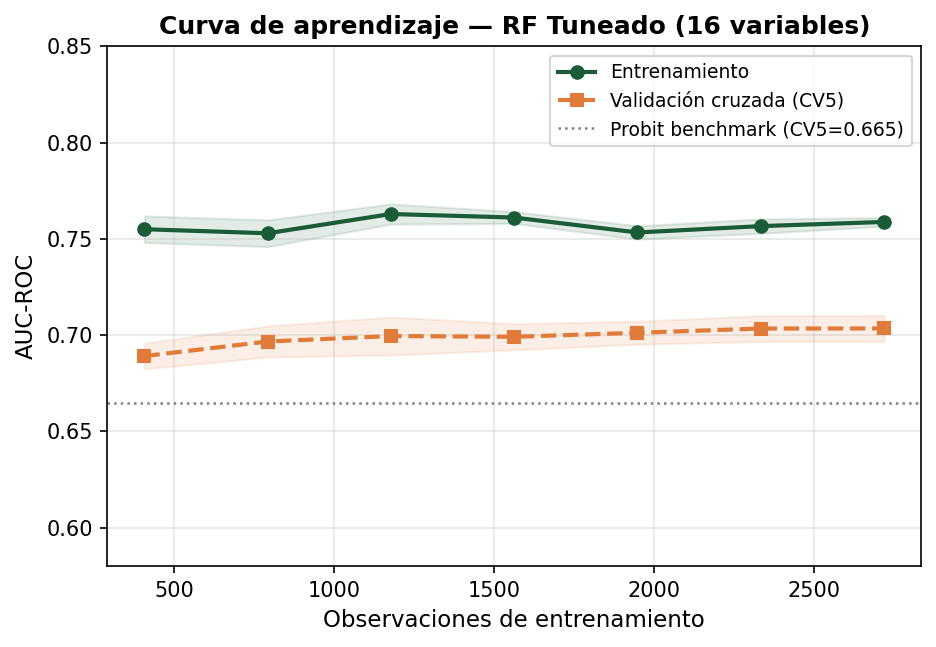
\includegraphics[width=0.82\textwidth]{../figures/curva_aprendizaje_rf.png}
\\
\vspace{0.15cm}
\scriptsize
Brecha \textit{train-CV5} estable en $\approx 0.057$ a lo largo del rango muestral.\\
Descarta memorización: el sobreajuste residual es el optimismo estructural del bagging sobre datos in-bag.\\
La curva de CV5 supera al benchmark Probit (línea punteada, 0.665) desde $n \approx 500$.
\end{frame}

% Interpretabilidad SHAP
\section{Interpretabilidad}

\begin{frame}
\frametitle{¿Por qué SHAP?}
\textbf{Problema}: el GBM es una caja gris. Sin interpretabilidad, no es útil para política pública.

\vspace{0.3cm}
\textbf{SHAP (Lundberg \& Lee, 2017)}: descompone cada predicción como suma de contribuciones por variable.

\vspace{0.2cm}
\textit{Propiedad clave}: aditividad
\[
f(x_i) = \phi_0 + \sum_j \phi_{ij}
\]

\vspace{0.2cm}
La importancia global es $\text{Imp}_j = \mathbb{E}[\,|\phi_j|\,]$.
\end{frame}

\begin{frame}
\frametitle{Importancia SHAP — global (modelo ampliado)}
\centering
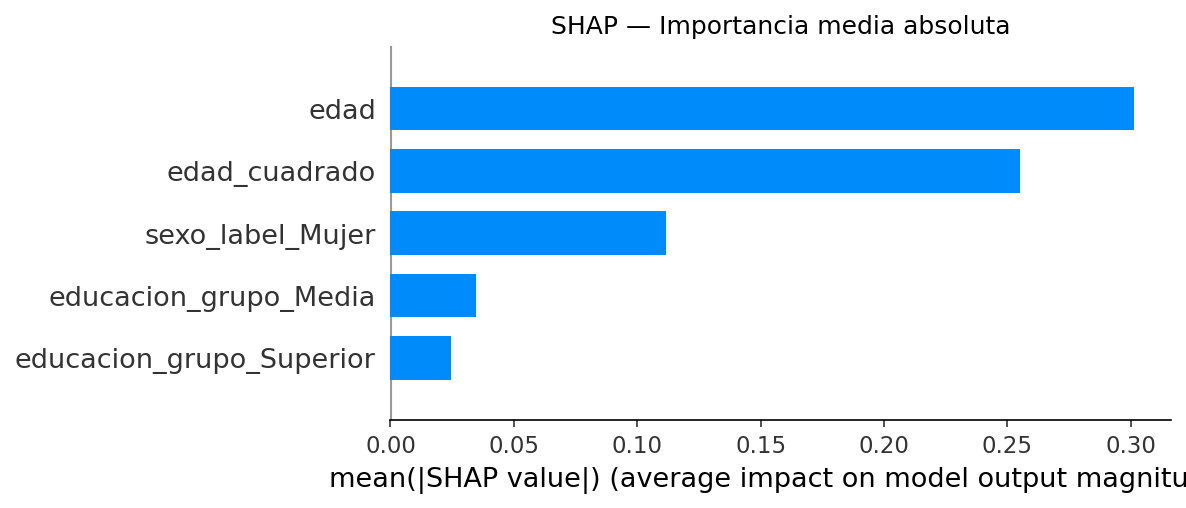
\includegraphics[width=0.78\textwidth]{../figures/shap_bar.png}
\\
\vspace{0.2cm}
\small Con 4 features: edad + edad² ${\sim}77\%$, sexo 15\%, educación 8\% — modelo demográfico puro.\\
Con 16 features: se espera que \texttt{amigos\_consumen}, \texttt{probaria\_sustancias} y \texttt{riesgo\_marihuana\_ocasional} ganen peso. Ver notebook 06 para el análisis actualizado.
\end{frame}

\begin{frame}
\frametitle{SHAP summary — distribución individual}
\centering
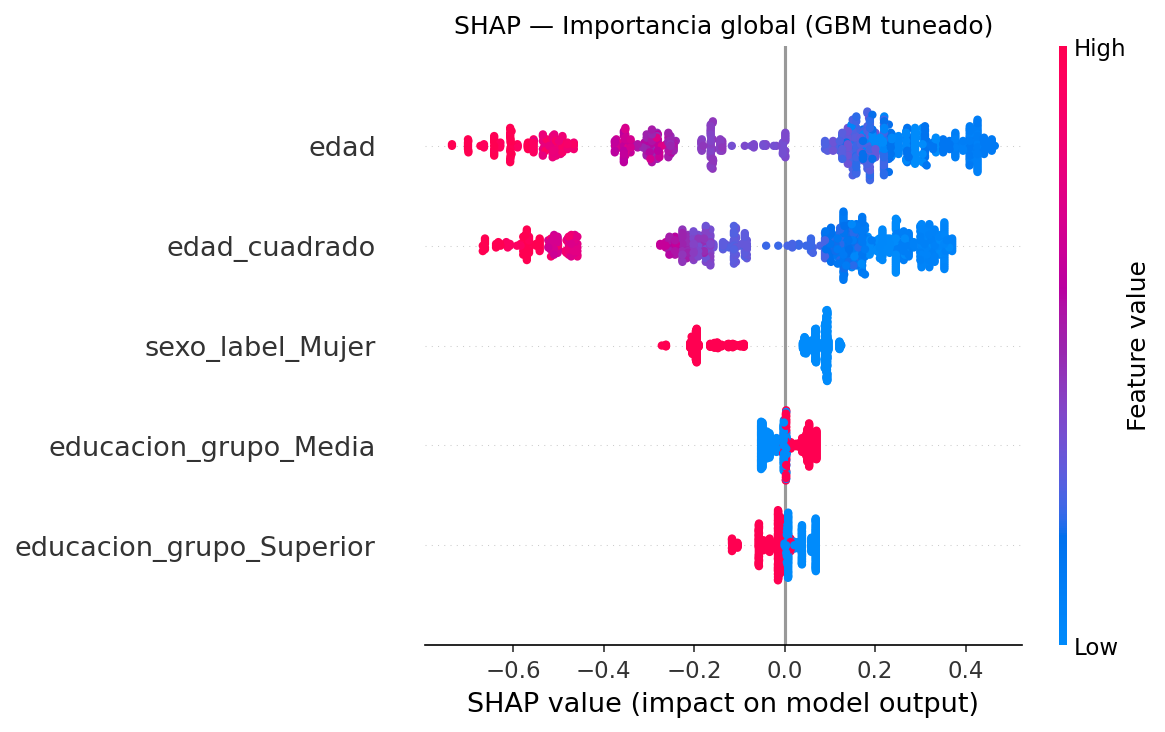
\includegraphics[height=0.78\textheight,keepaspectratio]{../figures/shap_summary.png}
\end{frame}

\begin{frame}
\frametitle{Dependencia parcial — edad}
\centering
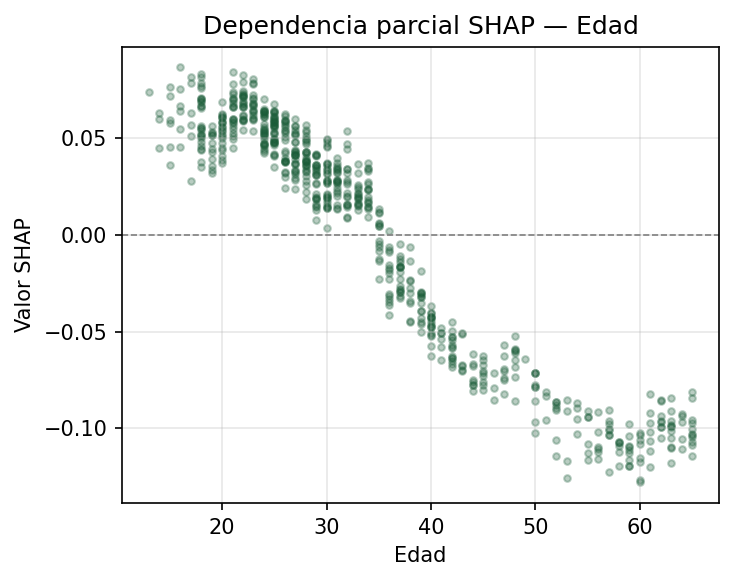
\includegraphics[height=0.66\textheight,keepaspectratio]{../figures/shap_dependence_edad.png}
\\
\vspace{0.05cm}
\scriptsize Relación no monótona: positiva en jóvenes, decae con la edad. Por qué gana el GBM: captura mejor esta forma funcional que el lineal.
\end{frame}

\begin{frame}
\frametitle{Robustez — Y alternativa estricta}
\small
\textbf{Motivación}: la auditoría detectó que \texttt{consumo\_12m} difiere de \texttt{K\_03} en 898 casos.

\vspace{0.2cm}
\textbf{Test}: reentrenar el GBM tuneado con $Y_{\text{alt}}=\mathbb{1}\{K\_03=1\}$.

\vspace{0.2cm}
\centering
\footnotesize
\begin{tabular}{lrrr}
\toprule
Métrica & Y original & Y estricta & $\Delta$ \\
\midrule
AUC-ROC (test)        & 0.7182 & 0.6870 & $-0.031$ \\
CV AUC-10fold (mean)  & 0.6685 & 0.6951 & $+0.027$ \\
\bottomrule
\end{tabular}
\vspace{0.25cm}
\\
\flushleft
\scriptsize\textbf{Conclusión}: las relaciones estructurales se mantienen; la discrepancia no domina el resultado.
\end{frame}

% Ética, sesgos y limitaciones
\section{Ética e implicaciones}

\begin{frame}
\frametitle{Sesgos del dato}
\begin{itemize}
    \item \textbf{Autoreporte y deseabilidad social}: el modelo aprende propensión a \emph{reportar}, no a \emph{consumir}. Subreporte correlacionado con percepción de riesgo legal.
    \item \textbf{Sesgo de selección por precio}: la submuestra con precio ($n\approx 755$) está sesgada hacia personas más expuestas al mercado.
    \item \textbf{Sesgo de medición en Y}: discrepancia documentada \texttt{consumo\_12m} vs \texttt{K\_03}. Mitigada con análisis de robustez.
\end{itemize}
\end{frame}

\begin{frame}
\frametitle{Riesgos del uso del modelo}
\begin{enumerate}
    \item \textbf{Perfilado individual}: AUC $\approx 0.73$ implica solapamiento alto entre grupos. \textit{No usar} para decisiones sobre personas (policial, laboral, escolar).
    \item \textbf{Asociaciones $\neq$ causalidad}: edad y sexo correlacionan con factores no observados (red social, entorno).
    \item \textbf{Estigma reforzado}: mapas y perfiles públicos refuerzan estereotipos. Privilegiar lecturas agregadas.
\end{enumerate}
\end{frame}

\begin{frame}
\frametitle{Uso responsable propuesto}
\textbf{Sí} (uso agregado):
\begin{itemize}
    \item Estimar tamaño de mercado bajo escenarios regulatorios.
    \item Diseño tributario simulando bases de contribuyentes por estratos amplios.
    \item Priorizar segmentos para política preventiva.
\end{itemize}
\vspace{0.3cm}
\textbf{No} (uso individual):
\begin{itemize}
    \item Decisiones sobre personas específicas.
    \item Focalización geográfica fina sin análisis de equidad.
    \item Predicciones puntuales sin intervalos de incertidumbre.
\end{itemize}
\end{frame}

\begin{frame}
\frametitle{Implicaciones de política}
\textbf{Diseño tributario}:
\begin{itemize}
    \item Base concentrada en cohortes jóvenes-masculinas.
    \item Elasticidad-precio probablemente alta $\Rightarrow$ impuesto excesivo desplaza al mercado ilegal.
    \item Recaudo creíble requiere acoplar este modelo con una elasticidad estimada limpia.
\end{itemize}
\vspace{0.3cm}
\textbf{Política preventiva}:
\begin{itemize}
    \item Focalizar en 18--25 años, diferenciada por sexo.
    \item Aprovechar la sensibilidad de la cohorte a intervenciones tempranas.
\end{itemize}
\end{frame}

% Conclusiones
\section{Conclusiones}

\begin{frame}
\frametitle{Hallazgos clave}
\begin{enumerate}
    \item El benchmark MCO/Probit alcanza AUC-ROC = 0.7232. Es un piso difícil de superar con sólo 4 \textit{features}.
    \item Los modelos ML por defecto \textit{no} superan al benchmark.
    \item El \textbf{GBM tuneado} sí lo hace: AUC = \textbf{0.7278}, F1 = \textbf{0.6129}.
    \item SHAP: edad + edad² $\approx 77\%$ de la importancia. Modelo \emph{honestamente delgado}.
    \item Robustez Y alternativa: relaciones estructurales estables.
\end{enumerate}
\end{frame}

\begin{frame}
\frametitle{Lecciones metodológicas}
\begin{itemize}
    \item La flexibilidad sin regularización introduce varianza que opaca la ganancia de sesgo.
    \item El \textit{tuning} disciplinado importa más que el algoritmo en datos chicos.
    \item La interpretabilidad no es opcional: define qué tan utilizable es el modelo para política.
    \item Documentar limitaciones (Y discrepante, submuestra con precio) es parte del trabajo, no un anexo.
\end{itemize}
\end{frame}

\begin{frame}
\frametitle{Próximos pasos}
\begin{itemize}
    \item Reconciliar la construcción de \texttt{consumo\_12m} con \texttt{K\_03} directo.
    \item Ampliar el \textit{feature set} con variables de entorno (geografía, red social, ingreso del hogar).
    \item Estimar elasticidad-precio con un diseño que corrija el sesgo de selección.
    \item Acoplar el modelo de propensión con proyecciones poblacionales del DANE para simulación tributaria.
\end{itemize}
\end{frame}

\begin{frame}[plain]
\centering
\Huge \textbf{Preguntas y discusión}
\vspace{0.6cm}
\\[0.4cm]
\normalsize
\textit{Tupaz, Quintero, Rodrigues — Universidad EAFIT}\\
\textit{Profesora supervisora: Paula María Almonacid Hurtado}
\end{frame}


\end{document}

